\subsection{Lo Stato Patrimoniale}
Rappresenta la situazione aziendale alla chiusura dell’esercizio: in tale prospetto deve essere evidenziata la situazione \textit{patrimoniale} e \textit{finanziaria} della società che compone l’attivo, quella che compone il passivo e, come differenza tra le due, il patrimonio netto. Lo stato patrimoniale è suddiviso in due sezioni: attivo e passivo.

\textit{Attivo} – Tutti i beni e le proprietà possedute dall’azienda (fabbricati, macchinari, attrezzature) utilizzati per l’esercizio dell’attività, i crediti dell’azienda nei confronti di terzi (clienti, etc.), le disponibilità liquide (cassa, saldi attivi dei conti correnti).

\textit{Passivo} – Debiti dell’azienda verso terzi (fornitori, banche, ...). Il capitale netto indica il debito ideale della società verso i suoi proprietari, ed è costituito dalle riserve e dal capitale sociale.

\begin{table}[H]
	\begin{tabular}{| c | c |}
		\hline
		 Attivo & Passivi e Netto \\
		 \hline
		 Beni e diritti a disposizione & Insieme dei diritti di terzi nei \\
		 dell’impresa per realizzare l’attività &  confronti dell’impresa \\
		 & \\
		 Investimenti in attività & FONTI di finanziamento ricevute \\
		 (IMPIEGHI delle risorse) &  dall’impresa: \\ 
		 & - Passività di terzi \\ 
		 & - Capitale Netto \\
		 \hline
	\end{tabular}
	\centering
	\caption{Schema Stato Patrimoniale}
\end{table}

\begin{figure}[H]
	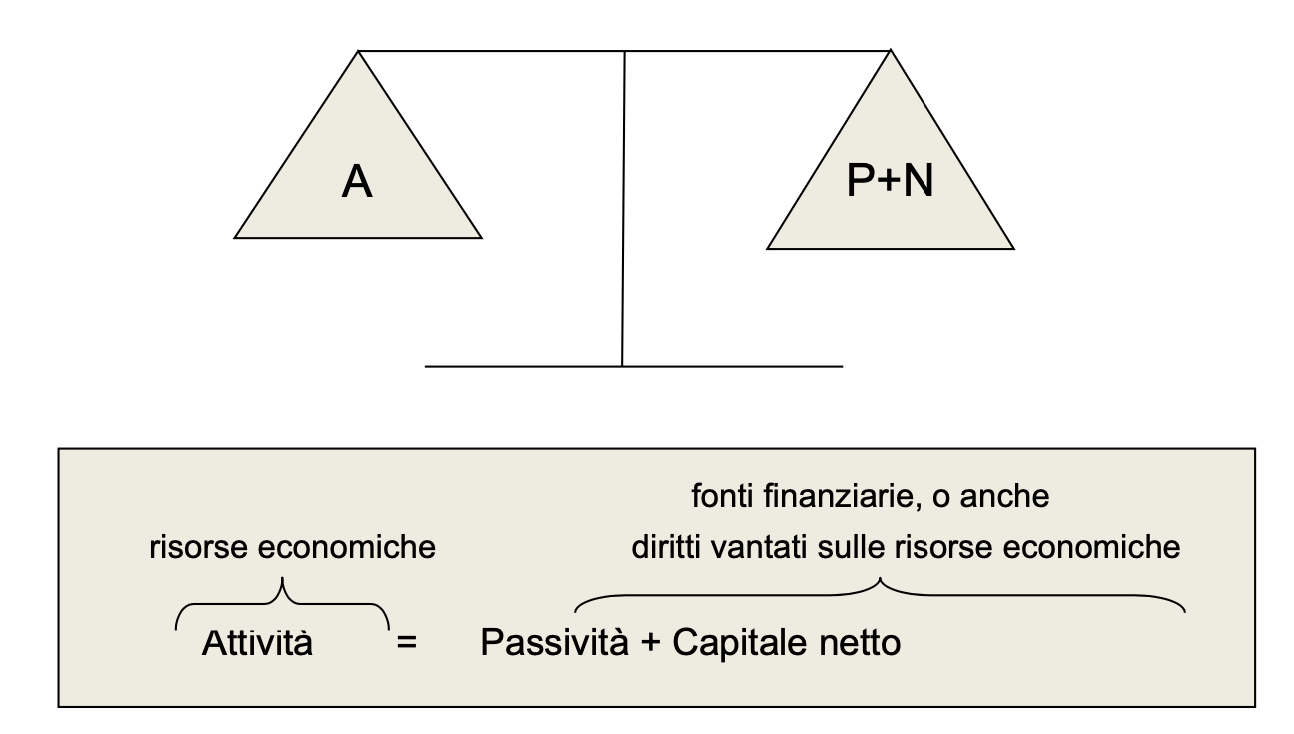
\includegraphics[width=0.8\linewidth]{resources/chapters/Bilancio/images/equazione-bilancio.png}
	\centering
	\caption{Equazione di bilancio}
\end{figure}

\subsubsection{L'attivo}